\documentclass[12pt, a4paper]{article}

\usepackage[T1,T2A]{fontenc}
\usepackage[utf8]{inputenc}
\usepackage[english,russian,ukrainian]{babel}
\usepackage[pdftex]{graphicx}
\usepackage{graphicx, hyperref, float, caption}
\usepackage{amsmath, amssymb, amsthm}
\usepackage{titlesec, indentfirst, listings, fancyhdr, enumitem}
\usepackage{etoolbox,xpatch}
\usepackage{minted, tikz}
\usetikzlibrary{positioning}

\paperwidth=210mm
\paperheight=297mm

\hoffset=-5.0mm
\voffset=-20.4mm

\oddsidemargin=0mm
\evensidemargin=0mm

\textwidth=180mm
\textheight=257mm

\setminted[python]{
    autogobble=true,
    frame=lines,
    framesep=3mm,
    fontsize=\footnotesize
}

\makeatletter
\AtBeginEnvironment{minted}{\dontdofcolorbox}
\def\dontdofcolorbox{\renewcommand\fcolorbox[4][]{##4}}
\xpatchcmd{\inputminted}{\minted@fvset}{\minted@fvset\dontdofcolorbox}{}{}
\makeatother

\renewcommand{\labelenumii}{\theenumii}
\renewcommand{\theenumii}{\theenumi.\arabic{enumii}.}

\begin{document}
\begin{titlepage}

\center

\textsc{\Large Київський національний університет імені Т. Шевченка \\
Факультет комп’ютерних наук та кібернетики}\\[7.5cm] 
	
	{\huge\bfseries Моделювання систем}\\[0.4cm]
	
	{\large\bfseries Лабораторна робота 3}\\[0.4cm]
	
    \vfill\vfill
	
	\begin{minipage}{0.8\textwidth}
		\begin{flushright}
			\large
			\textbf{Виконав}\\
			студент групи ІС-31 \\
			А.С. \textsc{Хома}
		\end{flushright}
	\end{minipage}

   \vfill
	
	{\large \textbf{ Київ-2018}} 

\end{titlepage}

\section*{Умова}

Будемо вважати, що на вхід системи перетворення, математична модель якої невідома, поступають послідовно дані у вигляді $m-1$  вимірних векторів $x_j$. На виході системи спостерігається сигнал у вигляді вектора $y_j$ розмірності $p$.

\begin{center}
  \begin{tikzpicture}
    \node (rect) at (0,0) [draw,thick,minimum width=2cm,minimum height=1cm] (a) {P};

    \draw[<-] (a.west) --++(0:-1.5cm) node [above,pos=0.5] {$x_j$};
    \draw[->] (a.east) --++(0:1.5cm) node [above,pos=0.5] {$y_j$};
  \end{tikzpicture}

\end{center}

\section*{Хід роботи}

\begin{enumerate}
  \item Реалізуємо псевдообернення по Муру-Пенроузу та за Гревілем.
  \begin{enumerate}
    \item Псевдообернення по Гревілю.
    \inputminted[firstline=24, lastline=46]{python}{pseudo-inverse-python.py}
    \pagebreak
    \item Псевдообернення по Муру-Пенроузу.
    \inputminted[firstline=49, lastline=68]{python}{pseudo-inverse-python.py}
  \end{enumerate}
  \item Обрахуємо перетворення для обох методів.
  \inputminted[firstline=71, lastline=81]{python}{pseudo-inverse-python.py}
  \item Перетворимо початкове зобреження $X$ в $Y$.
  \inputminted[firstline=87, lastline=97]{python}{pseudo-inverse-python.py}
  \pagebreak
  \item Виведемо отримані результати. \\
  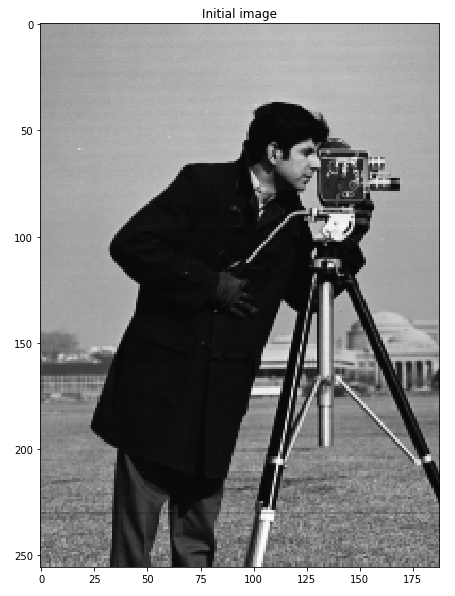
\includegraphics[scale=0.39]{initial_1.png}
  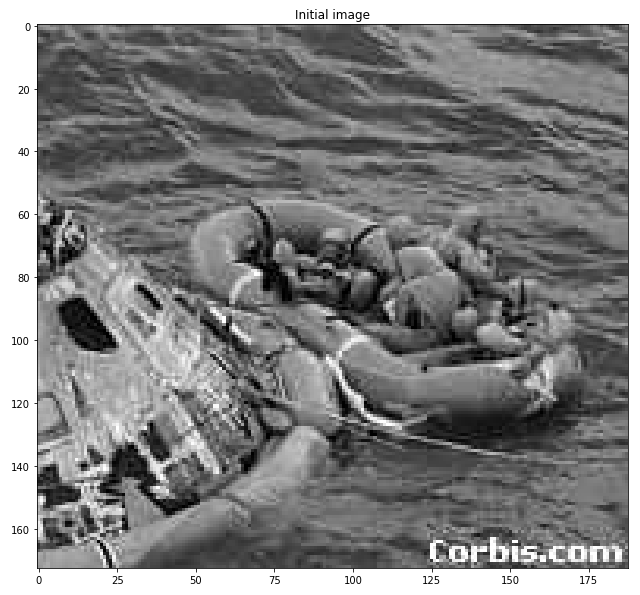
\includegraphics[scale=0.39]{initial_2.png} \\
  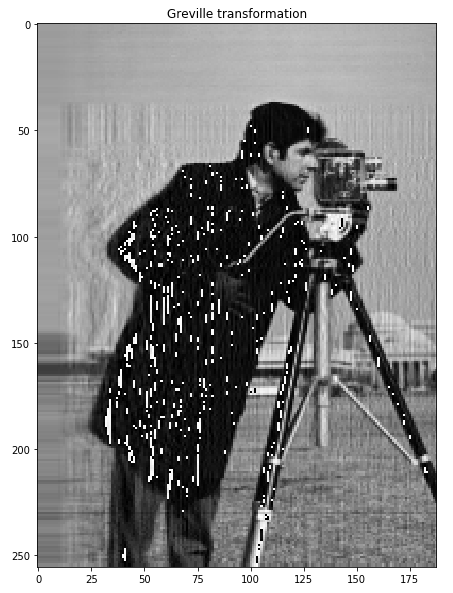
\includegraphics[scale=0.39]{Greville_1.png}
  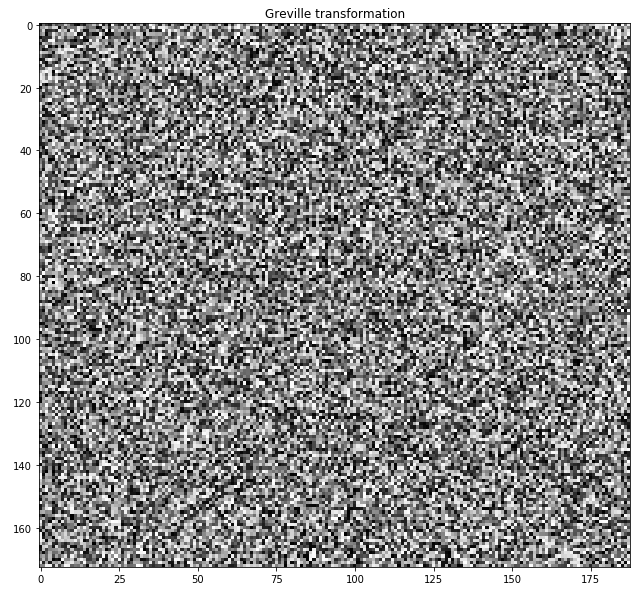
\includegraphics[scale=0.39]{Greville_2.png} \\
  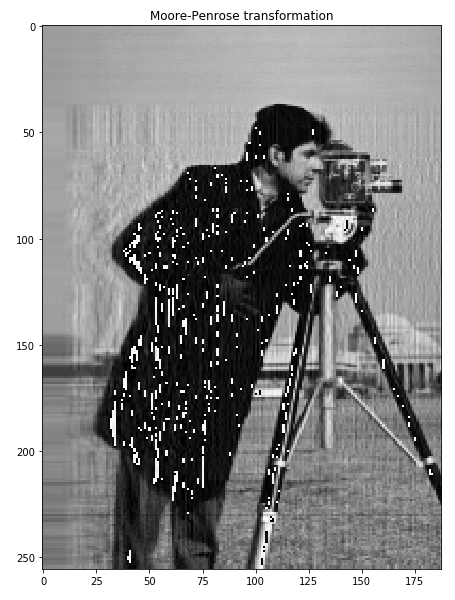
\includegraphics[scale=0.39]{Moore_1.png}
  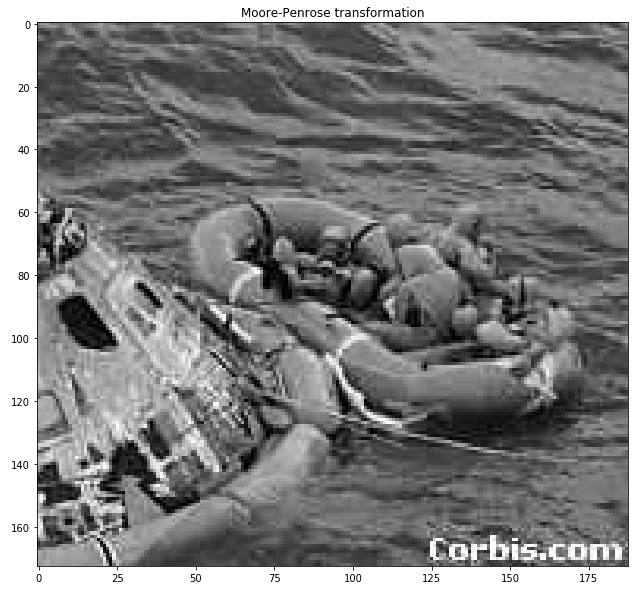
\includegraphics[scale=0.39]{Moore_2.png}
\end{enumerate}

\end{document}